\subsection{排序}
Rust的整数型数组和向量(Vector)的排序是相同的,可以使用相同的方式进行,即采用
sort以及sort\_unstable进行。其中,sort是稳定排序(即不重新排序相等的元素),
sort\_unstable是不稳定排序,\colorunderline{但是通常情况下速度更快},并且不会进行辅助内存的分配。
\begin{code-block}{rust}
let mut v = vec![2, 21, 12, 32, 12, 45, 90];
v.sort_unstable();
info!("The sorted vector is {:?}", v);
let mut array = [2, 23, 12, 12, 98, 100, 21];
array.sort_unstable();
info!("The sorted array is {:?}", array);
\end{code-block}
默认情况下,排序操作使用的是升序,但是可以通过定制,修改排序方式:
\begin{code-block}{rust}
let mut v = vec![2, 21, 12, 32, 12, 45, 90];
// 降序排列,可替换成v.sort_by
v.sort_unstable_by(|a, b| b.cmp(a));
info!("The sorted vector is {:?}", v);
let mut array = [2i32, -23, 12, 12, 98, -100, 21];
// 根据绝对值升序排列,可以根据其他关键字进行排序
array.sort_unstable_by_key(|k| k.abs());
info!("The sorted array is {:?}", array);
// 根据字符顺序排列,带有缓存cache,闭包函数通常只执行一次,比无缓存的快速
let mut xx = [-5i32, 4, 32, -3, 2];
xx.sort_by_cached_key(|k| k.to_string());
// 字符串排序
let mut array = ["lucifer", "titans", "asura", "garuda"];
array.sort_unstable_by_key(|item| item.to_string());
info!("The string array is {:?}", array);
let mut array = [
    "lucifer".to_string(),
    "titans".to_string(),
    "asura".to_string(),
    "garuda".to_string(),
];
// 可以转换成切片
// array[..].sort_unstable_by_key(|item| item.to_string());                                                                                                                               info!("The string array is {:?}", array);
array.sort_unstable_by_key(|item| item.to_string());                                                                                                                               info!("The string array is {:?}", array);
\end{code-block}

浮点数的排序和最值操作,参见\colorunderlineref{float_sort}

除了基础数据类型可以进行排序,同样可以针对复合数据类型进行排序。在针对复合数据
类型排序时,需要实现\colorunderline{Eq,PartialEq,Ord和PartialOrd}这几个trait:
\begin{code-block}{rust}
#[derive(Eq, PartialEq, Ord, PartialOrd, Debug)]
struct Student {
    name: String,
    age: u8,
}
fn main() {
    let mut stu = [
        Student {
            name: "lucifer".to_string(),
            age: 18,
        },
        Student {
            name: "garuda".to_string(),
            age: 36,
        },
    ];
    // 按照自然序列(name)
    stu.sort();
    info!("The students is {:?}", stu);
    // 根据年龄
    stu.sort_unstable_by(|first, second| first.age.cmp(&second.age));
    info!("The students is {:?}", stu);
}
\end{code-block}

\subsection{压缩与解压}
Rust可以实现文件的压缩与解压,在Linux环境下,通常使用\href{https://github.com/alexcrichton/tar-rs}{tar}(归档)
和\href{https://github.com/rust-lang/flate2-rs}{flate2}(压缩解压),比如Linux下常见的tar.gz文件的处理:
\begin{code-block}{rust}
use flate2::read::GzDecoder;
use flate2::write::GzEncoder;
use flate2::Compression;
use tar::Archive;

let path = "/root/py3.tar.gz";
let targz = match File::open(path) {
    Ok(file) => file,
    Err(error) => {
        crit!("Failed to open the file {}: {}", path, error.to_string());
    }
};
// gz文件的解码器
let tar = GzDecoder::new(targz);
// tar的管理器
let mut archive = Archive::new(tar);
// 将tar.gz解压
match archive.unpack(".") {
    Ok(_) => info!("Sucess to unpack the tar.gz file"),
    Err(error) => {
        crit!("Failed to unpark the tar.gz file: {:?}", error);
    }
}
// 创建tar.gz文件
let targz = match File::create("log.tar.gz") {
    Ok(file) => file,
    Err(error) => {
        crit!(
            "Failed to create the log.tar.gz file : {}",
            error.to_string()
        );
    }
};
// 创建gz文件的编码器,压缩算法使用默认
let encoder = GzEncoder::new(targz, Compression::default());
let mut tarfile = tar::Builder::new(encoder);
// 将文件添加到tar.gz文件当中
match tarfile.append_dir_all("log", "/var/log") {
    Ok(_) => info!("log.tar.gz created sucessful"),
    Err(error) => {
        fs::remove_file("log.tar.gz").unwrap_or_else(|why| {
            error!("Cannot remove the log.tar.gz: {:?}", why.to_string())
        });
        crit!("Failed to park the tar.gz file: {:?}", error);
    }
}
\end{code-block}

当然,归档和压缩也可以单独使用:
\begin{code-block}{rust}
use flate2::read::GzDecoder;
use flate2::write::GzEncoder;
use flate2::Compression;
use tar::Archive;
let tarf = match File::create("log.tar") {
    Ok(file) => file,
    Err(error) => {
        crit!("Failed to create the log.tar file : {}", error.to_string());
    }
};
// 注意和gz文件不一样,只是归档,则不需要创建编码器
let mut tar_file = tar::Builder::new(tarf);
match tar_file.append_dir_all("log", "/var/log") {
    Ok(_) => info!("log.tar created sucessful"),
    Err(error) => {
        fs::remove_file("log.tar")
            .unwrap_or_else(|why| error!("Cannot remove the log.tar: {:?}", why.to_string()));
        crit!("Failed to park the tar.gz file: {:?}", error);
    }
}
let path = "/root/log.tar";
let tarball = match File::open(path) {
    Ok(file) => file,
    Err(error) => {
        crit!("Failed to open the file {}: {}", path, error.to_string());
    }
};
// 同样的,解压tar文件,不需要创建解码器
let mut archive = Archive::new(tarball);
match archive.unpack(".") {
    Ok(_) => info!("Sucess to unpack the tar file"),
    Err(error) => {
        crit!("Failed to unpark the tar file: {:?}", error);
    }
}
\end{code-block}

\section{元编程}
Rust也包含了宏,并且,和C/C++相比,Rust的宏会展开成为抽象语法树(AST,abstract syntax tree),
而不是普通的转换成字符串,因此,不会产生无法预料的优先权错误。最普通的宏如下:
\begin{code-block}{rust}
extern crate slog_scope;
extern crate slog_stdlog;
#[macro_use]
extern crate log;
extern crate logger;

// macro_rules! 表示后续的内容是一个宏
// greeting表示宏的名称
macro_rules! greeting {
    // () 表示该宏不接收任何参数
    () => {
        // 宏定义展开的具体内容
        info!("hello macro");
    };
}

fn main() {
    let logger = logger::initlogger(false, "", 0);
    let _guard = slog_scope::set_global_logger(logger);
    slog_stdlog::init().unwrap();

    greeting!();
}
\end{code-block}
但是,宏不可能一直是无参数的,它还包含了多种使用方式。宏的参数使用\$符号表示,并
使用指示符来注明类型,如下:
\begin{code-block}{rust}
macro_rules! create_function {
    // 宏接收一个ident指示符表示的参数,并创建一个func_name的函数
    // ident指示符表示变量名(函数名)
    ($func_name: ident) => {
        fn $func_name() {
            // stringify宏负责将ident指示符表示的参数转换成字符串
            info!("You called the {}()", stringify!($func_name));
        }
    };
}

// 使用宏创建函数,函数名为func
create_function!(func);

macro_rules! formatres {
    // 宏接收一个expr指示符表示的表达式(可以是代码块,函数/方法,其他宏)
    // expr指示符表示表达式
    // $expression表示表达式最后的执行结果
    ($expression: expr) => {
        info!("{} = {}", stringify!($expression), $expression)
    };
}

fn main() {
    // 调用func函数
    func();
    formatres!(1 + 32);
    formatres!("lucifer");
    formatres!(format!("{}, age is {}", "zhangjl", 32));
}
\end{code-block}
宏的指示符有很多,各自用于不同的场景,所有的宏指示符如下:
\begin{itemize}
  \item block:代码块,由{}限定的代码
  \item expr:表达式,会生成具体的值
  \item ident:变量名/函数名,标识符
  \item item:语言项,即组成一个Rust包的基本单位,如模块,声明,函数/类型/结构体/impl定义
  \item pat:模式
  \item path:路径,类似std::iter等
  \item stmt:语句,一般以;结尾的代码
  \item tt:标记树
  \item ty:类型
  \item meta:元数据信息,即包含在\#[...]以及\#![...]当中的信息
  \item vis:可见性,如pub
  \item lifetime:指代生命周期参数
\end{itemize}

类似于方法,Rust的宏也可以进行重载,只不过,这个重载的实现比较类似于match的分支
处理流程,分割宏的分支即进行重载,则需要使用符号“:”进行:
\begin{code-block}{rust}
macro_rules! assert_bool {
    // 括号中的分号;表示调用该宏时,需要传递2条语句或者表达式
    ($left: expr; and $right: expr) => {
        info!(
            "{} and {} is {}",
            stringify!($left),
            stringify!($right),
            $left && $right
        )
    };
    // 分支之间需要使用分号;进行分割与结束
    ($left: expr; or $right: expr) => {
        info!(
            "{} or {} is {}",
            stringify!($left),
            stringify!($right),
            $left || $right
        )
    };
}

fn main() {
    assert_bool!(1 + 1 == 2; and 2 * 2 == 4 );
    assert_bool!(1 + 1 == 3; or 2 * 2 == 6 );
}
\end{code-block}

宏定义的另外一个好处就是可以处理不定参数,在处理不定参数时,需要使用+操作符以及*
操作符,+表示参数可能出现一次或多次,*则表示参数可能出现0次或多次:
\begin{code-block}{rust}
use std::cmp;
macro_rules! find_min {
    // 如果传入的只有一个参数,直接返回当前参数值
    ($x: expr) => {
        $x
    };
    // 传入多个参数,表示后续更多的参数,即x后至少还有一个参数
    ($x: expr, $($y: expr), +) => {
        // 递归调用宏本身
        cmp::min($x, find_min!($($y), +))
    };
}

fn main() {
    info!("{}", find_min!(12));
    info!("{}", find_min!(12, 65, 40 - 32));

    let a = 1;
    let b = 2;
    let c = 3;
    info!("{}", find_min!(a, a - b, c));
}
\end{code-block}
上述的宏是使用表达式模式进行的,如果采用变量模式,即使用ident模式,则上述代码需要
变更为如下:
\begin{code-block}{rust}
use std::cmp;

macro_rules! find_min {
    ($x: ident) => {
        $x
    };
    ($x: ident, $($y: ident), +) => {
        cmp::min($x, find_min!($($y), +))
    };
}

fn main() {
    // 错误的使用方式,12是一个表达式,而并非变量名
    // info!("{}", find_min!(12));
    let a = 1;
    let b = 2;
    let c = 3;
    info!("{}", find_min!(a, b, c));
}
\end{code-block}
通过对比,可以发现,在某些场景下,表达式方式比ident方式更加通用,也更加合理一些。

比较奇特的是,在Rust的宏当中,可以使用自定义的关键字,实现特殊功能,比如自定义
关键字evaluation,表示将表达式进行计算:
\begin{code-block}{rust}
macro_rules! calc {
    // 自定义关键字evalution,使用该宏时,前面必须加上evalution前缀关键词
    (evalution $e: expr) => {
        // 强制将表达式e变成数值i32类型,即将表达式e进行计算
        let val: i32 = $e;
        info!("{} = {}", stringify!($e), val);
    };
    // 当传入参数不定时
    (evalution $e: expr, $(evalution $es: expr),+) => {
        calc!(evalution $e);
        calc!($(evalution $es),+)
    }
}

fn main() {
    calc!(evalution 1 + 100);
    calc!(evalution 1+2, evalution 3 + 4, evalution 5 +6 );
    calc!(evalution 1-2, evalution 3 * 4, evalution (5 +6) * (5 - 9) );
}
\end{code-block}
由于宏的高度可定制性,因此,上述的宏代码可以变更为如下的模式,但是2者的功能完全
一样:
\begin{code-block}{rust}
macro_rules! calc {
    (evalution $e:expr) => {{
        let val: i32 = $e;
        info!("{} = {}", stringify! {$e}, val);
    }};
    (evalution $e:expr, $(evalution $es:expr),+) => {{
        calc! { evalution $e }
        calc! { $(evalution $es),+ }
    }};
}

fn main() {
    // 下面两种方式都正确
    calc!{evalution 1 + 100};
    calc!(evalution 1+2, evalution 3 + 4, evalution 5 +6 );
}
\end{code-block}

实际上,*和+不仅可以用于参数处理,也可以用于语法扩展的部分,比如,我们想实现类似
如下的一个宏:
\begin{code-block}{rust}
let empty = hashmap![];
let counts = hashmap!['A' => 0, 'C' => 0, 'G' => 0, 'T' => 0];
\end{code-block}
则宏定义大致可能如下:
\begin{code-block}{rust}
macro_rules! hashmap {
    ($key: expr => $val: expr) => {{
        let mut map = ::std::collections::HashMap::new();
        map.insert($key, $val);
        map
    }};
}
\end{code-block}
但是,到目前为止,上述的宏只能实现对一对数据的操作,无法实现任意对数据的插入操作,
因此,我们需要使用+或者*符号进行扩展,由于我们需要支持初始化一个空的hashmap,因此
选择使用*进行扩展:
\begin{code-block}{rust}
macro_rules! hashmap {
    ($key: expr => $val: expr) => {{
        let mut map = ::std::collections::HashMap::new();
        map.insert($key, $val);
        map
    }};
}
\end{code-block}
虽然参数支持了任意个数,但是,在宏体当中,map的插入操作只执行了一次,我们可以继续
使用*和+对语法部分进行扩展,扩展之后,完整的宏定义如下:
\begin{code-block}{rust}
macro_rules! hashmap {
    ($($key: expr => $val: expr), *) => {{
        let mut map = HashMap::new();
        $(map.insert($key, $val); )*
        map
    }};
}
\end{code-block}
使用时,则按照上述的使用方式即可:
\begin{code-block}{rust}
let map = hashmap!["lucifer" => 12, "titans" => 18];
let mut empty: HashMap<String, u8> = hashmap![];
\end{code-block}
默认情况下,cargo并没有提供将宏定义进行展开显示的功能,但是,我们可以通过rustc
将代码展开,确认宏定义确实是按照我们的想法进行工作的。只是需要注意,将宏定义进行
展开显示,需要使用nightly分支,因此,我们的操作基本如下:
\begin{code-block}{bash}
# 切换到nightly分支
rustup default nightly
# 对代码进行展开
rustc -Z unstable-options --pretty=expanded src/main.rs
cargo rustc -- -Z unstable-options --pretty=expanded
# 如果代码需要依赖其他的非std的crate的,则应当如下执行
# rustc -Z unstable-options --pretty=expanded -L ../target/debug/deps src/main.rs
\end{code-block}
如果一切正常,则我们调用宏的代码就会被展开成如下的形式:
\begin{figure}[H]
  \centering
  
\includegraphics[width=\linewidth]{rust_macro_expand.png}
  \caption{宏展开}
  \label{fig:rust_macro_expand}
\end{figure}

Rust宏的灵活性非常大,可以像C/C++一样,在宏当中嵌套/调用宏:
\begin{code-block}{rust}
macro_rules! serial_cmd {
    ($expression: expr, $port: expr, $item: expr, $timeout: expr) => {{
        let mut cmd = HEADER.to_vec();
        cmd.push($item);
        cmd.push($expression);
        match ($port).write(&cmd) {
            Ok(_) => info!(
                "Sucess {}(0x{:X>02}) the {} board, and command is {:?}",
                stringify!($expression),
                $expression,
                $item,
                &cmd
            ),
            Err(e) => error!(
                "Failed to {}(0x{:X>02}) the {} board: {}",
                stringify!($expression),
                $expression,
                $item,
                e
            ),
        }
        if 0 < $timeout {
            thread::sleep(Duration::from_secs($timeout));
        }
    }};
}

macro_rules! serial_for_all_cmd {
    ($expression: expr, $port: expr, $timeout: expr) => {{
        for item in &CODE {
            serial_cmd!($expression, $port, *item, $timeout);
        }
    }};
}
\end{code-block}
也可以直接在宏当中,插入语句块,作为宏执行的一部分:
\begin{code-block}{rust}
macro_rules! serial_for_only_one {
    ($port: expr, $location: expr, $($command: stmt),*) => {{
        serial_cmd!(POWEROFF, $port, $location, 0);
        trace!("Remove the block file to avoid the unexcepted error ...");
        let _ = fs::remove_file("/dev/sdb");

        serial_cmd!(SWITCH, $port, $location, 5);
        // 执行外部代码块
        $($command )*

        serial_cmd!(POWEROFF, $port, $location, 0);
        let _ = fs::remove_file("/dev/sdb");
    }};
}

fn main() {
    // 调用宏
    serial_for_only_one!(port, location_u8, {println!("hello")});
}
\end{code-block}

Rust的宏实际上属于元编程的一部分,除了在当前的crate当中使用宏之外,
宏还可以导出,宏之间也可以相互调用。宏的导出通常使用macro\_export关键字,比如:
\begin{code-block}{rust}
#[macro_export]
macro_rules! inc {
    ($x: expr) => {
       println!("{}", $x);
    };
}
\end{code-block}
然后,在其他地方,就可以直接使用这个宏。不过,有的时候,宏的实现可能需要当前包的
一些函数或者方法进行配合,则需要做如下的更改:
\begin{code-block}{rust}
// 必须将方法设置为pub,否则后续在宏定义当中,无法使用
pub fn incr(x: u32) -> u32 {
    x + 1
}

#[macro_export]
macro_rules! inc {
    ($x: expr) => {
        // $crate关键字表示当前的包
        // 当宏被导出时,自动根据上下文选择函数调用路径当中的包名
        $crate::incr($x)
    };
}
\end{code-block}
上述的导出方式,要求宏所依赖的函数,也都必须导出,否则,在外部使用宏时,无法
正常工作。

除了使用普通的函数作为宏的依赖项之外,也可以使用宏作为宏的依赖项。和普通函数一样,
如果一个宏的定义当中,依赖了另外一个宏,则必须同样当对应的依赖项导出为pub类型。
但是,如果可以使用一种额外的方式,将依赖的宏,转变为宏的内部规则进行导出:
\begin{code-block}{rust}
#[macro_export]
macro_rules! hashmap {
    /* hashmap宏的内部规则,相当于如下的一个外部宏,不管接收多少参数,一律返回
       一个空元组()
       macro_rules! unit {
       ($($input:tt),*) => {
                ()
           };
       }
       使用方式
       let res = unit!(), unit!("lucifer"), unit!("garuda", "titans")
    */
    (@unit $($x:tt)*) => (());

    /* hashmap宏的内部规则, 等价于如下的一个宏,作用是返回接收到的元素的个数
       macro_rules! count {
           // <[()]>::len()可以用于求取数组/切片的长度,使用方式如下:
           // let lenth = <[&str]>::len(&["string", "string"])
           // let lenth = <[String]>::len(&["string".to_string(), "string".to_string()])
           // let lenth = <[()]>::len(&[(), ()]) // 性能更好,因为()不占据任何内存空间
           ($($key:expr),*) => (<[()]>::len(&[$(unit! ($key)),*]));
       }
       使用方式
       let res = count!(), count!("lucifer"), count!("lucifer", "titans")

       @符号表示一个宏定义当中的内部规则,如果需要在宏当中使用宏的内部规则,
       则使用方式是 宏名!(@内部规则名 其他变量),对应到这个hashmap宏,则使用方式
       如下: hashmap!(@unit $key), hashmap!(@count $($rest),*)
    */
    (@count $($rest:expr), *) => (<[()]>::len(&[$(hashmap!(@unit $rest)),*]));

    /* $($key:expr => $value:expr),* 表达式本身可以匹配hashmap!(),hashmap!("1"=>2)
     但是,无法匹配类似hashmap!["2"=>3,]这种末尾包含,符号的模式
     $(,)* 则是用于匹配后续结尾是否带有,符号
     即hashmap!["2"=>3,]和hashmap!["2"=>3]都可以支持
    */
    ($($key:expr => $value:expr),* $(,)*) => {{
        let _cap = hashmap!(@count $($key),*);
        let mut _map = ::std::collections::HashMap::with_capacity(_cap);
        $( _map.insert($key, $value); )*
        _map
    }}
}
\end{code-block}

以上提到的宏,都是声明宏,可以直接当作函数/方法使用的类型,但是,如果想实现类似于
\#[derive(Debug)]这种类型的宏,声明宏是做不到的。相对应的,这种类型的宏则被称之
为过程宏。过程宏主要用于下面3种用途:
\begin{itemize}
  \item 自定义派生属性:即类似于\#[derive(Debug)]这样的derive属性
  \item 自定义属性:即类似于实现\#[cfg()]这样的属性
  \item Bang宏:与声明宏类似,但是,是以!结尾的宏,可以当作函数/方法使用
\end{itemize}

过程宏要求必须放到proc\_macro类型的lib包当中,因此,过程宏的创建过程会稍微有一些
区别:
\begin{code-block}{bash}
cargo new --lib procmacro
echo -e "[lib]\nproc_macro=true" >> procmacro/Cargo.toml
\end{code-block}

另外,和其他的mod不太一样的是,过程宏的测试用例,不能放到相同的crate当中,必须以
外部的方式存在,因此,过程宏的文件结构大致如下:
\begin{code-block}{bash}
├── Cargo.toml
├── src
│   └── lib.rs
└── tests
    └── test.rs
\end{code-block}

实现derive方式的过程宏,其示例如下:
\begin{code-block}{rust}
// 必须如此进行使用
extern crate proc_macro;
use self::proc_macro::TokenStream;

#[proc_macro_derive(A)]
pub fn derive(input: TokenStream) -> TokenStream {
    let input = input.to_string();
    assert!(input.contains("struct A"));
    r#"
        impl A {
            pub fn a(&self) -> String {
                format!("Hello from impl A")
            }
        }
    "#
    .parse()
    .unwrap()
}
\end{code-block}
上述过程宏表示,使用\#[derive(A)]为结构体A实现一个a方法,方法直接输出一句话。相对应的,
测试用例当中的使用则应当修改如下:
\begin{code-block}{rust}
#[macro_use]
extern crate procmacro;

#[derive(A)]
struct A;
#[test]
fn test_derive_a() {
    assert_eq!("Hello from impl A", A.a());
}
\end{code-block}

而实现自定义属性宏稍微有些区别,就是必须在nightly的rust下编译,目前还没有进入到
stable分支,一个简单的示例如下:
\begin{code-block}{rust}
#![feature(register_attr)]
extern crate proc_macro;
use self::proc_macro::TokenStream;

#[proc_macro_attribute]
pub fn attr_with_args(args: TokenStream, _: TokenStream) -> TokenStream {
    let args = args.to_string();
    //let input = input.to_string();
    format!("fn foo() -> &'static str {{{}}}", args)
        .parse()
        .unwrap()
}
\end{code-block}
同样的,其测试用例如下:
\begin{code-block}{rust}
#![feature(register_attr)]
#[macro_use]
extern crate procmacro;
use procmacro::attr_with_args;

#[attr_with_args("Hello Rust")]
fn foo() {}

#[test]
fn test_foo() {
    assert_eq!("Hello Rust", foo());
}
\end{code-block}
原本的foo方法,不接收参数,同样没有返回值,但是,在attr\_with\_args这个过程宏
当中,将其强行修改为了一个返回为字符串切片的函数。

实现Bang宏的方式则如下:
\begin{code-block}{rust}
#![feature(proc_macro_hygiene)]
extern crate proc_macro;
use self::proc_macro::TokenStream;

#[proc_macro]
pub fn treemap(input: TokenStream) -> TokenStream {
    let input = input.to_string();
    let input = input.trim_end_matches(',');
    let input_v: Vec<String> = input
        .split(",")
        .map(|n| {
            let mut data = if n.contains(":") {
                n.split(":")
            } else {
                n.split("=>")
            };
            let (key, value) = (data.next().unwrap(), data.next().unwrap());
            format!("hm.insert({}, {})", key, value)
        })
        .collect();
    let count: usize = input.len();
    let token = format!(
        "{{
        let mut hm = ::std::collections::HashMap::with_capacity({});
        {}
        hm
    }}",
        count,
        input_v
            .iter()
            .map(|n| format!("{};", n))
            .collect::<String>()
    );
    token.parse().unwrap()
}
\end{code-block}

Bang宏可以如同声明宏一样的进行使用,其使用方式如下:
\begin{code-block}{rust}
#[macro_use]
extern crate procmacro;

#[test]
fn test_treemap() {
    let hm = treemap! {"a":1, "b": 2};
    assert_eq!(hm["a"], 1);
    let hm = treemap! {"a" => 1, "b" => 4};
    assert_eq!(hm["b"], 4);
}
\end{code-block}

过程宏的本质是在函数/方法当中,使用TokenStream重构,本质还是一个特殊的函数/方法。
因此,过程宏不需要像声明宏一样的进行export,但是,必须将过程宏的函数声明为pub,
生成的过程宏才可以被外部使用。

\section{并发/并行/异步}
Rust也同样支持常见的并行和并发操作,也同样分为进程,线程以及消息通信等等。

\subsection{线程}
Rust的线程操作必须使用闭包完成。在之前看到的闭包当中,通常采用的都是有参的闭包,
而在Rust的线程操作当中,则经常会遇到无参数的闭包;Rust的线程使用thread::spawn函数
进行实现:
\begin{code-block}{rust}
use std::thread;
use std::time::Duration;
fn main() {
    thread::spawn(|| {
        for i in 1..10 {
            println!("hi number {} from the spawned thread!", i);
            thread::sleep(Duration::from_millis(1));
        }
    });
    for i in 1..5 {
        println!("hi number {} from the main thread!", i);
        thread::sleep(Duration::from_millis(1));
    }
}
\end{code-block}
和其他语言的线程概念一样,当主线程结束时,所有的线程都会被终止。因此上述代码当中,
子线程(spawn)无法将所有的循环执行完成。为了达成所有进/线程执行完成之后才退出主
进/线程的目的,和其他的开发语言相同,需要在主进程当中调用join函数:
\begin{code-block}{rust}
fn main() {
    let handle = thread::spawn(|| {
        for i in 1..10 {
            println!("hi number {} from the spawned thread!", i);
            thread::sleep(Duration::from_millis(1));
        }
    });
    for i in 1..5 {
        println!("hi number {} from the main thread!", i);
        thread::sleep(Duration::from_millis(1));
    }
    handle.join().unwrap();
}
\end{code-block}
Thread::spawn的返回值是JoinHandle,是一个拥有所有权的值,当对其调用join方法时,
它会等待对应线程结束;而join的返回值是一个Result,可以按照之前介绍的方式进行处理。
同时,Join函数是一个阻塞式函数,只有当该函数运行结束之后,才会继续进行后续的操作。

多数情况下,Rust的线程不可能只会在内部运行,而和外部没有数据交互。但是,如果我们
直接使用外部数据,则会出现错误,比如下方的代码:
\begin{code-block}{rust}
fn main() {
    let v = vec![1, 2, 3];
    let handle = thread::spawn(|| {
        println!("Here's a vector: {:?}", v);
    });
    handle.join().unwrap();
}
\end{code-block}
\begin{figure}[H]
  \centering
  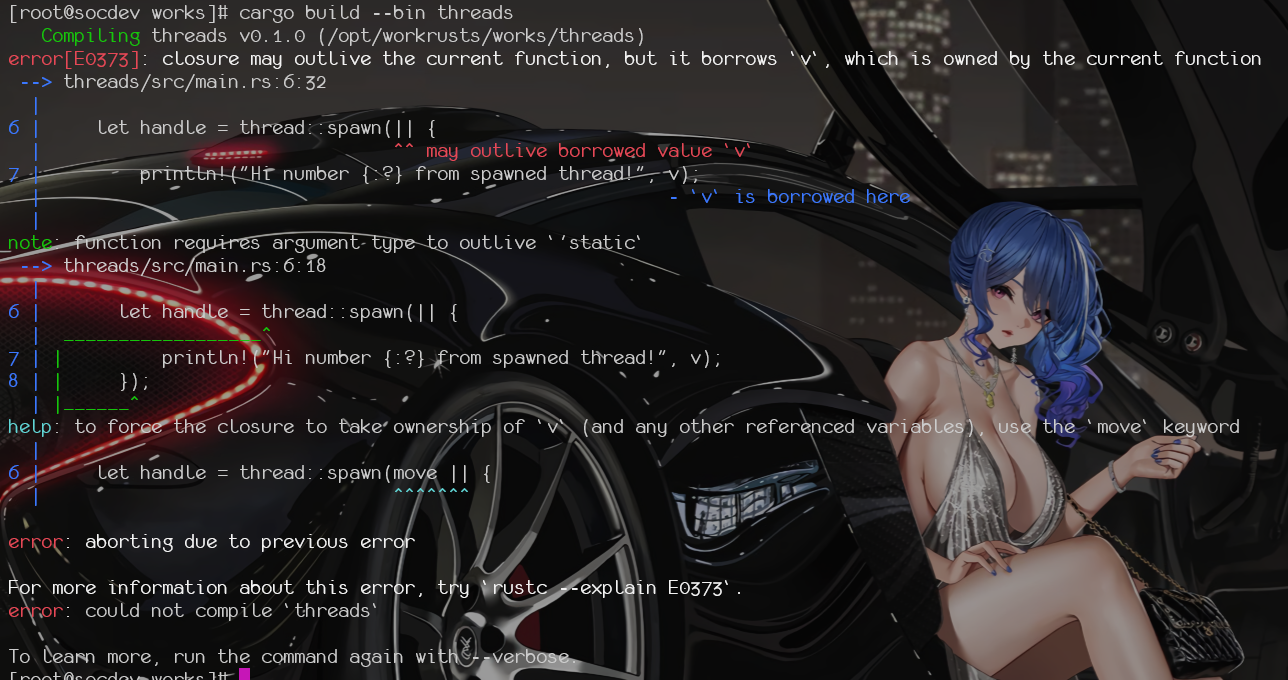
\includegraphics[width=\linewidth]{rust_thread_out_params.png}
  \caption{试图访问线程外部资源}
  \label{fig:rust_thread_out_params}
\end{figure}
线程使用的是闭包,从闭包的定义来说,是可以捕获并使用外部变量和数据的;但是,Rust
不知道这个线程到底会运行多长时间,因此无法知道对外部变量的引用是否一直有效,比如
下方的代码:
\begin{code-block}{rust}
fn main() {
    let v = vec![1, 2, 3];
    let handle = thread::spawn(|| {
        println!("Here's a vector: {:?}", v);
    });
    drop(v);
    handle.join().unwrap();
}
\end{code-block}
启动线程的同时,立即将v进行丢弃,线程内部无法知道v在运行阶段是否继续有效,就会
出现错误,因此,如果在线程当中使用默认的闭包模式,则无法对应的闭包是无法捕获以及
使用外部的变量和数据的。此时,则需要使用move闭包进行替换,即强制闭包获取外部变量
的所有权,而不是由Rust进行借用推断。但是需要注意,一旦使用move之后,在线程之外,
变量将无法再进行使用:
\begin{code-block}{rust}
fn main() {
    let v = vec![1, 2, 3];
    let handle = thread::spawn(move || {
        println!("Here's a vector: {:?}", v);
    });
    // 下方代码无法再进行执行
    // println!("{:?}", v);
    handle.join().unwrap();
}
\end{code-block}

\subsection{消息通信和消息传递}
每个线程做自己的事情,但是,不管什么编程语言,都需要考虑线程之间的数据交互问题。
Rust向Golang进行了学习,使用通信替换共享内存,来进行线程之间的数据传输。同样的,
Rust当中用于消息传递并发的主要工具是通道,该概念和Golang的通道概念相同。Rust的通道
分为2个角色:发送者和接收者,发送者发送消息,接收者接收消息,当发送者或者接收者任一
被丢弃时,则对应的通道被视为关闭。

Rust的通道采用mpsc::channel函数实现,mpsc表示多个生产者,单个消费者,因此,Rust
标准库实现通道的方式意味着一个通道可以有多个产生值的发送(sending)端,但只能有
一个消费这些值的接收(receiving)端。通道的实现示例如下:
\begin{code-block}{rust}
use std::sync::mpsc;
fn main() {
    let (sender, recevier) = mpsc::channel();
}
\end{code-block}
其中,函数的第一个返回值为发送者,第二个参数为接收者。使用通道发送数据通信的示例
如下:
\begin{code-block}{rust}
use std::sync::mpsc;
use std::thread;
fn main() {
    let (sender, recevier) = mpsc::channel();
    thread::spawn(move || {
        let val = "lucifer".to_string();
        match sender.send(val) {
            Ok(_) => println!("Send success"),
            Err(error) => println!("Send failed :{:?}", error),
        }
    });
    let res = match recevier.recv() {
        Ok(s) => s,
        Err(error) => {
            println!("Cannot recevie anything from sender: {:?}", error);
            "".to_string()
        }
    };
    println!("The result of channel is {}", res);
}
\end{code-block}
接收者接收消息有2种模式:默认的recv是阻塞式,返回一个Result<T, E>,当通道关闭时,
将返回Result当中的Error;而try\_recv是非阻塞式,同样是返回一个Result<T, E>,但是,
Result当中的Error表示没有接收到任何消息,可以使用for循环进行反复的尝试读取操作。
另外需要注意的是,Send函数会改变变量的所有权,当该函数执行之后,被发送的消息
(变量)将无法再使用。

但是,通道可以反复使用,而且和Golang的类似,Rust的通道也是可以进行迭代的,特别
是在接收消息时,通常采用for循环进行操作,减少了错误处理的代码,使得代码更具可读性:
\begin{code-block}{rust}
use std::sync::mpsc;
use std::thread;
fn main() {
    let (sender, recevier) = mpsc::channel();

    let handler = thread::spawn(move || {
        let vals = vec!["lucifer", "titans", "garuda"];
        for val in vals {
            match sender.send(val) {
                Ok(_) => println!("Send success"),
                Err(error) => println!("Send failed :{:?}", error),
            }
        }
    });
    for msg in recevier {
        println!("The msg is {}", msg);
    }
    match handler.join() {
        Err(error) => println!("Error{:?}", error),
        _ => (),
    }
}
\end{code-block}

同样的,由于Rust的通道默认是多生产者/单消费者,因此,可以通过多个发送端向单个接
收端发送消息。实际使用当中的多个发送端,则通常是某个发送端的克隆对象,如下:
\begin{code-block}{rust}
use std::sync::mpsc;
use std::thread;
fn main() {
    let (sender, recevier) = mpsc::channel();
    let sender_copy = sender.clone();

    let handler = thread::spawn(move || {
        let vals = vec!["lucifer", "titans", "garuda"];
        for val in vals {
            match sender.send(val) {
                Ok(_) => println!("Send success"),
                Err(error) => println!("Send failed :{:?}", error),
            }
        }
    });
    let handler_copy = thread::spawn(move || {
        let vals = vec!["zhangjl", "luoyan", "zhangzz"];
        for val in vals {
            match sender_copy.send(val) {
                Err(error) => println!("Send failed :{:?}", error),
                _ => (),
            }
        }
    });
    for msg in recevier {
        println!("The msg is {}", msg);
    }
    match handler_copy.join() {
        Err(error) => println!("Error{:?}", error),
        _ => (),
    }
    match handler.join() {
        Err(error) => println!("Error{:?}", error),
        _ => (),
    }
}
\end{code-block}

\subsection{共享状态}
在其他语言当中,有些特殊的场景,还是必须使用原有的线程并发概念——锁——来进行资源的
访问/读写控制。Rust当中同样存在锁,比较常见的就是互斥锁(互斥器,Mutex)以及原子
计数器(Arc)。在基本的操作上,互斥锁的使用和其他语言当中没有太大的区别:
\begin{code-block}{rust}
use std::sync::Mutex;
fn main() {
    let m = Mutex::new(5);
    {
        let mut num = m.lock().unwrap();
        *num = 6;
    }
    println!("m = {:?}", m);
}
\end{code-block}
注意,上述代码如果将内部大括号去除,则运行结束之后,m的状态还是锁定状态;但是,
有大括号,则表示大括号内部的段是一个有效的生命周期,当该生命周期结束之后,互斥
锁将自动释放。一旦获取了锁,就可以将返回值(在这里是num)视为一个其内部数据的
\colorunderline{可变引用}。类型系统确保了我们在使用m中的值之前
获取锁:Mutex<i32>并不是一个i32,所以必须获取锁才能使用这个i32值。

实质上,Mutex是一个智能指针,lock调用返回一个叫做MutexGuard的智能指针。这个智能
指针实现了Deref来指向其内部数据;同时也提供了一个Drop实现,使得MutexGuard离开作
用域时自动释放锁,即锁的释放是自动发生的。

但是默认情况下,Mutex是无法用于进行线程间的数据共享,如下:
\begin{code-block}{rust}
use std::rc::Rc;
use std::sync::Mutex;
use std::thread;
fn main() {
    let counter = Rc::new(Mutex::new(0));
    let mut handles = vec![];
    for _ in 0..10 {
        let counter = Rc::clone(&counter);
        let handle = thread::spawn(move || {
            let mut num = counter.lock().unwrap();
            *num += 1;
        });
        handles.push(handle);
    }
    for handle in handles {
        handle.join().unwrap();
    }
    println!("Result: {}", *counter.lock().unwrap());
}
\end{code-block}
上述代码会出现下面的类似错误:
\begin{figure}[H]
  \centering
  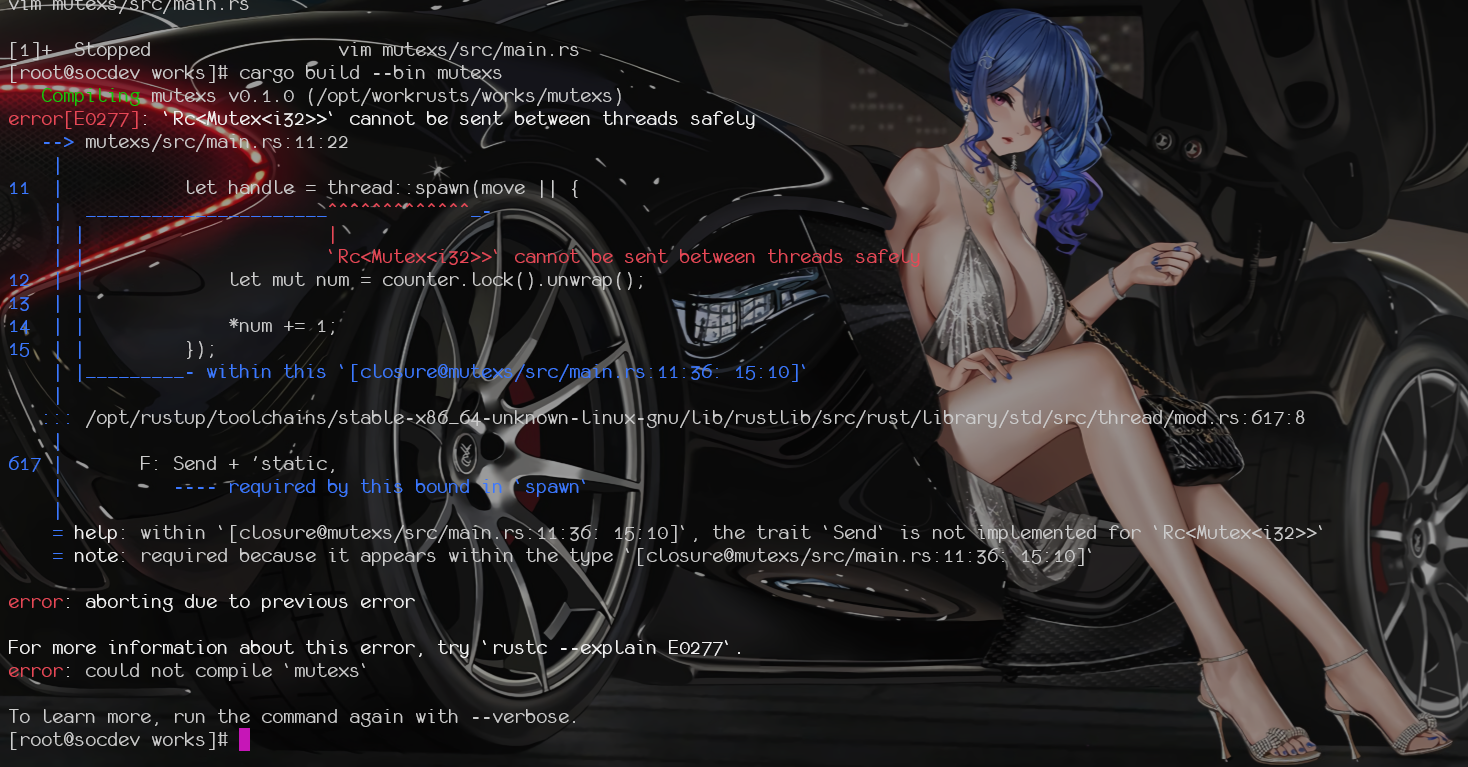
\includegraphics[scale=0.215]{rust_mutex_share_error.png}
  \caption{试图通过Rc共享Mutex的数据}
  \label{fig:rust_mutex_share_error}
\end{figure}
即之前提到的,Rc类型只能用于单线程/单进程环境。

而共享引用计数则需要使用Arc,它是可以安全的用于并发环境的类型,即原子引用计数,
可以在线程间进行共享所有权。Arc和Rc有相同的API,基本使用方法上类似。所有,可以直
接对上述代码进行修改:
\begin{code-block}{rust}
use std::sync::{Arc, Mutex};
use std::thread;
fn main() {
    let counter = Arc::new(Mutex::new(0));
    let mut handles = vec![];
    for _ in 0..10 {
        let counter = Arc::clone(&counter);
        let handle = thread::spawn(move || {
            let mut num = counter.lock().unwrap();
            *num += 1;
        });
        handles.push(handle);
    }
    for handle in handles {
        handle.join().unwrap();
    }
    println!("Result: {}", *counter.lock().unwrap());
}
\end{code-block}
通过这样简单的修改,成功实现了10个进程当中对同一个数值进行加法操作的功能。

虽然Rust本身的线程/进程管理非常完善,但是,thread::spawn产生的线程没有名称,并且
其栈空间大小默认为2M,如果需要需要针对线程/进程进行粒度更细的操作,比如自定义
线程名称,自定义线程的资源等等,此时,就需要使用thread::Builder进行修改,具体示例
如下:
\begin{code-block}{rust}
let mut v_thread = vec![];
for id in 1..5 {
    let thread_name = format!("child-{}", id);
    let size: usize = 1024;
    // 定义线程的名称,设置线程占用的栈大小为1M(1024)
    let builder = Builder::new().name(thread_name).stack_size(size);
    // builder.spawn返回的是Result<JoinHander, std::io::Error>
    // 需要进行处理,取出真正的线程句柄
    match builder.spawn(move || {
        info!(
            "In the child: {}, and the child name is {}",
            id,
            current().name().unwrap()
        );
    }) {
        Ok(child) => v_thread.push(child),
        Err(error) => error!("Cannot create the thread {} because: {:?}", id, error),
    };
}
// 其他的同普通的线程,
for child in v_thread {
    child.join().unwrap();
}
\end{code-block}

由于线程包含自己的资源空间,因此,存在一个特殊的存储空间——线程本地存储(Thread Local Storage,TLS),
存放在该区域的资源,其他线程无法访问,而是每个线程独占的数据:
\begin{code-block}{rust}
use std::cell::RefCell;
use std::thread;
fn main() {
    // 在线程本地存储定义一个FOO变量,最终的类型是thread::LocalKey
    thread_local!(static FOO: RefCell<u32> = RefCell::new(1));
    // 提供了一个with方法,可以通过给该方法传入闭包
    // 来操作线程本地存储中包含的变量
    FOO.with(|f| {
        info!("The f borrow is {}", *f.borrow());
        *f.borrow_mut() = 2;
    });
    let handler = thread::spawn(move || {
        // 子线程也有一个线程本地存储实例FOO,为主线程的副本
        // 也可以使用thread_local!宏在该子线程中重新创建一个LocalKey实例
        FOO.with(|f| {
            info!("In the handler thread The f borrow is {}", *f.borrow());
            *f.borrow_mut() = 3;
        });
    });
    // 主线程当中FOO实例并没有被子线程修改为3
    // thread local!宏定义单个线程内的一些独享数据
    FOO.with(|f| {
        info!("The f borrow is {}", *f.borrow());
    });
    handler.join().unwrap();
}
\end{code-block}

在同步原语支持方面,Rust也有自己的实现方式,通过使用std::thread当中的park函数提供
阻塞线程的能力,但并不能永久的阻塞线程,存在时间限制;而std::thread::part\_timeout
则可以显式的指定阻塞的超时时间;std::thread::Thread::unpark则可以将阻塞的线程重启;
如果需要让出当前线程的时间片,则需要使用std::thread::yeild\_now,让其他线程进行执行。
简单的阻塞例子如下:
\begin{code-block}{rust}
use std::thread::{self, Builder};
use std::time::Duration;
fn main() {
    let parked_thread = Builder::new()
        .spawn(|| {
            info!("Parking the thread ...");
            // 阻塞当前线程
            thread::park();
            info!("Thread parked");
        })
        .unwrap();
    thread::sleep(Duration::from_secs(5));
    info!("Unparking the thread");
    // 从JoinHandle中得到具体的线程
    parked_thread.thread().unpark();
    // 将该线程重新启动,该线程会继续沿着之前暂停的上下文执行
    parked_thread.join().unwrap();
}
\end{code-block}

除了常见的互斥锁(Mutex)之外,Rust也支持读写锁(RwLock)。读写锁的基本示例如下:
\begin{code-block}{rust}
use std::sync::RwLock;
fn main() {
    let rw_lock = RwLock::new(5);
    // 读写锁的使用必须使用{}进行区分,即便是单独使用读或者写也是一样
    // 通过代码块{},让读写锁自动释放,否则会出现死锁
    {
        let read_1 = rw_lock.read().unwrap();
        let read_2 = rw_lock.read().unwrap();
        info!("The read_1 is {}, and read_2 is {}", read_1, read_2);
    }
    {
        let mut write = rw_lock.write().unwrap();
        *write = 100;
    }
    info!("The data is {:?}", rw_lock);
}
\end{code-block}

而针对于同步的需求,Rust提供了屏障(Barrier)和条件变量(Condition Variable)原语。
屏障,是要求所有的条件全部满足之后,再进行后续操作,即在满足某个条件前,阻塞全部的
线程,通常用于线程同步,如下:
\begin{code-block}{rust}
use std::sync::{Arc, Barrier};
use std::thread;
fn main() {
    let mut vec = vec![];
    let barrier = Arc::new(Barrier::new(5));
    for id in 0..5 {
        let barrier_copy = barrier.clone();
        vec.push(thread::spawn(move || {
            info!("Thread {} Waiting the other threads...", id);
            // wait阻塞了所有的线程,当所有线程的wait之前部分全部执行完成之后
            // wait操作才算执行完成,才会执行每个线程后续的操作
            barrier_copy.wait();
            info!("{} After wait...", id);
        }));
    }
    for handler in vec {
        handler.join().unwrap();
    }
}
\end{code-block}

而条件变量与屏障稍微的区别在于,它不是阻塞所有的线程,而是在满足特定条件前,阻塞
一个得到了互斥锁的线程,如下:
\begin{code-block}{rust}
use std::sync::{Arc, Condvar, Mutex};
use std::thread;
use std::time::Duration;
fn main() {
    // 生成包含互斥锁的条件变量condvar
    let pair = Arc::new(((Mutex::new(false)), Condvar::new()));
    let pair_clone = pair.clone();
    let handler = thread::spawn(move || {
        let &(ref lock, ref cvar) = &*pair_clone;
        // 获得互斥锁
        let mut started = lock.lock().unwrap();
        info!("In the child thread");
        thread::sleep(Duration::from_secs(5));
        *started = true;
        // 通知主线程
        cvar.notify_one();
    });
    let &(ref lock, ref cvar) = &*pair;
    let mut started = lock.lock().unwrap();
    while !*started {
        info!("Waiting for the started singal {} ...", started);
        // 使用条件变量的wait阻塞当前线程,一直到cvar退出
        started = cvar.wait(started).unwrap();
        info!("Started singal finished {} ...", started);
    }
    handler.join().unwrap();
}
\end{code-block}
相比于单纯的互斥锁必须多次出入临界区才能获取到某个状态的信息,条件变量减少了系统
资源的浪费,但是需要注意,每个条件变量每次只能和一个互斥锁(体)一起使用。

除了使用锁、屏障以及条件变量,关于同步的问题,还可以使用原子操作。Rust目前只提供了
4个原子操作类型:AtomicBool、Atomiclsize、AtomicPtr和AtomicUsize。需要注意,虽然原子
操作类型本身可以保证操作的原子性,但是其本身并没有提供跨线程的共享方法,如果需要
使得原子数据类型也可以在线程间共享,则应当使用Arc进行封装,比如下面,使用原子类型
实现一个自旋锁:
\begin{code-block}{rust}
use std::sync::atomic::{AtomicUsize, Ordering};
use std::sync::Arc;

fn main() {
    let spinlock = Arc::new(AtomicUsize::new(1));
    let spinlock_clone = spinlock.clone();
    let handler = thread::spawn(move || {
        // 将原子类型的数据设置为0
        spinlock_clone.store(0, Ordering::SeqCst);
    });

    // 使用spinlock的load方法读取其内部原子类型的值,如果不为0,
    // 则不停地循环测试锁的状态,直到其状态被置为0为止
    // 所谓“自旋”就是指在语义上表示这种不断循环获取锁状态的行为
    while spinlock.load(Ordering::SeqCst) != 0 {}
    handler.join().unwrap();
}
\end{code-block}
代码当中的Ordering表示内存参数顺序,可以通过该参数来控制底层线程执行顺序。默认的,
Rust支持5种内存顺序,归为3大类:
\begin{itemize}
  \item 排序一致性顺序——SeqCst:最简单直观,要求必须先存储,后读取,在多线程环境下,所有的原子写操作都必须在读操作之前完成,强行指定了线程的执行顺序,保证了多线程中所有操作的全局一致性,但是存在性能损耗,其实质类似于餐厅点餐,相当于强制要求所有需要结账的客人,必须等所有点单的客户完成之后才可以结账
  \item 自由顺序——Relaxed:和SeqCst相反,完全不会对线程的顺序进行干涉,线程只进行原子操作,但是,线程之间会存在竞态条件,使用这种内存顺序会比较危险,只有在明确了解当前使用场景且必须使用它的情况下(比如只有读操作),才可使用自由顺序
  \item 获取-释放顺序——Release,Acquire和AcqRel: 是除排序一致性顺序之外的优先选择,默认情况下,不会对全部线程进行统一强制性的执行顺序要求,store表示释放(release),而load表示获取(acquire),通过这2种操作的协作实现线程同步。Release表示使用该顺序的store操作,之前所有的操作对于使用Acquire顺序的load操作都可见;反之,使用使用Aquire顺序的load操作,对于使用Release的store操作都是可见的;AcqRel表示读时使用Acquire顺序的load操作,写时使用Release顺序的store操作。获取释放顺序虽然不像排序一致性顺序那样对全局线程统一排序,但是它让每个线程都能接固定的顺序执行。
\end{itemize}

在此之前,已经谈到Rust支持channel通信来解决多线程环境所遇到的问题,比如之前的小例子:
\begin{code-block}{rust}
use std::thread;
use std::sync::mpsc::channel;

fn main() {
    let (tx, rx) = channel();
    let handler = thread::spawn(move || {
        tx.send(10).unwrap();
    });

    let res = rx.recv().unwrap();
    handler.join().unwrap();
}
\end{code-block}
像这种只有2个线程间通信的channel,称之为流通道,在流通道的内部,默认使用的是单生产者
单消费者的模式来提升性能。在此之前,我们看到多个发送者(生产者)单个接收者(消费者)
模式的通道,则称之为共享通道。而由于统一使用的channel函数生成通道,这样的通道又
称之为异步通道,即所有的操作都可以异步的进行处理,不会出现线程阻塞的情况。

同步通道的例子则如下:
\begin{code-block}{rust}
use std::thread;
use std::sync::mpsc::sync_channel;

fn main() {
    // 创建缓冲区为1的同步通道
    let (tx, rx) = sync_channel(1);
    tx.send(1).unwrap();
    let handler = thread::spawn(move || {
        tx.send(2).unwrap();
    });

    let res1 = rx.recv().unwrap();
    info!("The result is {}", res1);
    let res2 = rx.recv().unwrap();
    info!("The result2 is {}", res2);
    handler.join().unwrap();
}
\end{code-block}
在上述代码当中,由于channel的缓冲区设置为1,所以,当第一条信息被消费(recv)之前,
后续的消息发送会被一直阻塞,直到缓冲区可用为止。

虽然channel解决了很多的多线程同步和共享问题,但是,channel并没有解决死锁的问题,
当设计不周到的时候,channel同样会出现死锁的问题:
\begin{code-block}{rust}
use std::thread;
use std::sync::mpsc::channel;
fn main() {
    let (tx, rx) = channel();
    let mut handlers = vec![];
    for i in 0..5 {
        let tc = tx.clone();
        let handler = thread::spawn(move || {
            tc.send(i).unwrap();
        });
        handlers.push(handler);
    }
    // 如果注释下面代码,主线程将一直不退出
    // drop(tx);
    for j in rx.iter() {
        info!("{:?}", j);
    }
    for handler in handlers {
        handler.join().unwrap();
    }
}
\end{code-block}
因为rx的iter方法会阻塞线程,只要tx还没有被析构,该迭代器就会一直等待新的消息,
只有tx被析构之后,迭代器才能返回None,从而结束退出main主线程。由于上述代码的tx
一直没有析构,所以迭代器依旧会进行等待,但是tx也没有发送信息,从而造成死锁的状态。
显式调用drop之后,死锁将不会存在。

\subsection{同/异步}
Rust目前的版本当中,异步/同步的支持相对较低,目前,\href{https://github.com/rust-lang/futures-rs}{Futures}
提供了async和await的完整实现,\href{https://github.com/tokio-rs/tokio}{Tokio}也提供了
比较完整的平台支持,\href{https://github.com/async-rs/async-std}{Async-Std}也提供了
相关的支持。多线程的劣势主要体现在操作系统调度开销,难度较大,线程切换以及
跨线程共享数据会产生很多的额外开销,这些就是异步并发(async/await)发挥作用的
重要场景。

\subsection{优秀的并发-Crossbeam}
默认情况下,Rust标准库的多线程并发是非常安全和方便的,但是,也存在一些特殊情况,
会导致标准库的多线程使用起来受到诸多的限制,比如,在递归函数当中使用多线程:
\begin{code-block}{rust}
use std::thread;
const THRESHOLD: usize = 4;
// 由于Rust的跨线程通信的限制,要求input参数必须是static的生命周期
pub fn find_max(input: &'static [i32]) -> Option<i32> {
    if input.len() <= THRESHOLD {
        return input.iter().cloned().max();
    }
    let middle = input.len() / 2;
    let (left, right) = input.split_at(middle);
    // 由于thread限制,必须使用move关键字
    let thread_left = thread::spawn(move || find_max(left));
    let thread_right = thread::spawn(move || find_max(right));
    let max_left = thread_left.join().unwrap().unwrap();
    let max_right = thread_right.join().unwrap().unwrap();
    Some(max_left.max(max_right))
}
fn main() {
    static ARRAY_REF: &[i32] = &[12, 3, 45, 98, 100, 23, 878, 8765, 123, -897, 866666, 1241];
    let res = find_max(ARRAY_REF);
    info!("The res is {:?}", res);
}
\end{code-block}
由于诸多的限制,上述代码当中,如果需要对多个数组进行排序,则这些数组必须使用static
关键字进行标识,无法处理普通的数组,并且最终会导致生成的二进制文件比较大。

除此之外,比如Rust的通道,只存在多生产者单消费者这一种模式,这也并不符合现实生活
当中的多生产者多消费者的模型。为了改进Rust的并行/并发,目前大多数的开发者使用
\href{https://github.com/crossbeam-rs/crossbeam}{Crossbeam}替代标准库的thread,
比如,上述的递归函数当中使用多线程,就可以修改为如下的模式:
\begin{code-block}{rust}
extern crate crossbeam;
pub fn find_max_crossbeam(input: &[i32]) -> Option<i32> {
    if input.len() <= THRESHOLD {
        return input.iter().cloned().max();
    }
    let middle = input.len() / 2;
    let (left, right) = input.split_at(middle);
    crossbeam::scope(|s| {
        let thread_left = s.spawn(|_| find_max_crossbeam(left));
        let thread_right = s.spawn(|_| find_max_crossbeam(right));
        let max_left = thread_left.join().unwrap().unwrap();
        let max_right = thread_right.join().unwrap().unwrap();
        Some(max_left.max(max_right))
    })
    .unwrap()
}
fn main() {
    static ARRAY_REF: &[i32] = &[12, 3, 45, 98, 100, 23, 878, 8765, 123, -897, 866666, 1241];
    let res = short_lived::find_max_crossbeam(ARRAY_REF);
    info!("The res is {:?}", res);
    let array = [
        12, 3, 45, 98, 100, 23, 878, 8765, 123, -897, 866666, 12411234,
    ];
    let res = short_lived::find_max_crossbeam(&array);
    info!("The res is {:?}", res);
}
\end{code-block}
通过这样修改的函数,不管是针对static生命周期的还是普通生命周期的数据,都能够自如的处理。

同样的,也可以对Rust标准库的通道(Channel)进行优化,此时,则需要配合使用
\href{https://github.com/crossbeam-rs/crossbeam}{Crossbeam-Channel}。比如下面的例子:
启动2个并行的通道,一个通道负责消息的生产发送,一个通道负责消息的接收和处理。

\section{超越Unsafe}
Rust屏蔽了一系列的不安全操作来换取应用程序的稳定性和可靠性,但是,可以通过关键字
unsafe,切换到不安全的运行环境当中,并且在unsafe的代码块当中运行。常见的不安全操作
如下:
\begin{enumerate}
  \item 解引用裸指针
  \item 使用不安全的方法/函数
  \item 访问/修改可变的静态变量
  \item 实现不安全的Trait
  \item 访问union的字段
\end{enumerate}
在使用的时候,原则需要明确:保持unsafe块尽可能小,将不安全代码封装进一个安全的
抽象并提供安全API是一种常见的安全操作和手段。

所谓的裸指针,和普通的指针和智能指针相比,存在如下的区别:
\begin{enumerate}
  \item 允许忽略借用规则,可以同时拥有不可变和可变的指针,或多个指向相同位置的可变指针
  \item 不保证指向有效的内存
  \item 允许为空
  \item 不能实现任何自动清理功能
\end{enumerate}
Rust当中存在2个裸指针:分别写作*const T(不可变)和*mut T(可变),其基本的定义方式
如下:
\begin{code-block}{rust}
let mut num = 5;
let r1 = &num as *const i32; // 不可变的裸指针
let r2 = &mut num as *mut i32; // 可变的裸指针
\end{code-block}

裸指针的定义是安全的,但是,它的使用是不安全的,因此裸指针的使用必须在unsafe块
当中:
\begin{code-block}{rust}
fn main() {
    let mut num = 5;
    let r1 = &num as *const i32;
    let r2 = &mut num as *mut i32;
    unsafe {
        *r2 = 10;
        // r1,r2和num都会变更为10
        println!("{},{}", *r1, *r2);
    }
}
\end{code-block}
同样的,unsafe也可以用于定义函数/方法,不过也需要在unsafe块当中使用;但是,unsafe
的方法可以作为安全方法进行导出,在使用时,则不需要使用unsafe进行标记:
\begin{code-block}{rust}
fn main() {
    let mut num = 5;
    // 定义裸指针
    let r1 = &num as *const i32;
    let r2 = &mut num as *mut i32;
    // 使用不安全的函数/方法
    unsafe {
        unsafe_change(r1, r2);
    }
    println!("{}", num);
    safe_change(r1, r2);
    println!("{}", num);
}
// 定义不安全的函数/方法
unsafe fn unsafe_change(r1: *const i32, r2: *mut i32) {
    *r2 = 10;
    println!("{},{}", *r1, *r2);
}
// 将不安全的函数/方法封装进安全的方法当中
fn safe_change(r1: *const i32, r2: *mut i32) {
    unsafe {
        *r2 = 100;
    }
}
\end{code-block}

作为不安全的一部分,某些时候直接在Rust当中调用C语言的类库可以获得更好的性能,此时,
则同样需要在unsafe块当中使用,比如在Rust当中调用标准C的abs(绝对值)函数:
\begin{code-block}{rust}
extern "C" {
    fn abs(input: i32) -> i32;
}
fn main() {
    unsafe {
        println!("The unsafe from C: {}", abs(-200));
    }
}
\end{code-block}
上述代码出现的extern关键字,有助于创建和使用外部函数接口(Foreign Function
Interface,FFI)。外部函数接口是一个编程语言用以定义函数的方式,其允许不同(外部)
编程语言调用这些函数。Extern块中声明的函数在Rust代码中总是不安全的,

特别需要注意的是,Rust当中的可变全局变量(static)同样是不安全的,需要在unsafe
代码块当中使用;而不可变的全局常量(const和static)则不需要在unsafe块当中;另外,
全局变量同样可以是任意数据类型的:
\begin{code-block}{rust}
use std::fmt;
struct Version {
    major: u8,
    minor: u8,
}
impl fmt::Display for Version {
    fn fmt(&self, f: &mut fmt::Formatter) -> fmt::Result {
        write!(
            f,
            "The version of this bin is {}.{}",
            self.major, self.minor
        )
    }
}
// 不可变的全局常量
const __CONST_NUM__: Version = Version { major: 1, minor: 4 };
const __VERSION__: &str = "v1.4.0";
static __NAME__: &str = "lucifer";
// 可变的全局变量
static mut __COUNTER__: u8 = 1;
fn main() {
    println!("{}", __CONST_NUM__);
    println!("{}", __NAME__);
    unsafe {
        println!("{}", __COUNTER__);
    }
}
\end{code-block}

但是,并不是所有情形都适合使用unsafe,Rust本身也无法从编译器层面,保证unsafe的
代码块是完全正确的,不会出现任何错误的。比如,我们在使用裸指针*const T和*mut T
的时候,如果不够仔细,非常容易造成错误的结果:
\begin{code-block}{rust}
let mut y: u32 = 1;
let x = 1_i32;
// 将y转换成u32的裸指针,再转换成i32的裸指针,最后转换成i64的裸指针
let raw_mut = &mut y as *mut u32 as *mut i32 as *mut i64;
unsafe {
    // 对裸指针进行修改,类似于C/C++当中对指针数据的操作
    *raw_mut = -1;
}
info!("The x is {:X} and y is {:X}", x, y);
\end{code-block}
按照我们本来的设想,x会保持不变,始终为1,而y则可能变换成其他的数值,但是,实际
的结果却如下:
\begin{figure}[H]
  \centering
  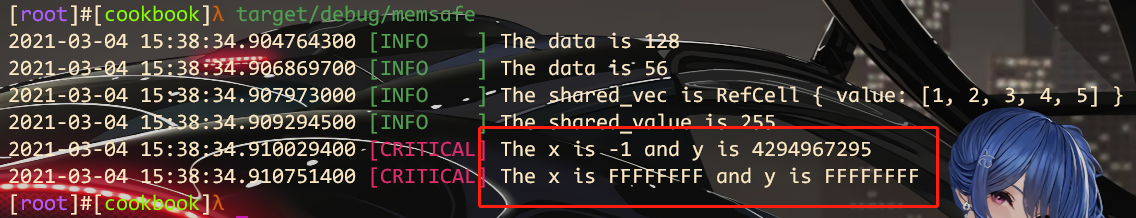
\includegraphics[width=\linewidth]{rust_raw_pointer.png}
  \caption{具有潜在错误的裸指针示例}
  \label{fig:rust_raw_pointer}
\end{figure}
x变成和y一样的值的原因在于:对指向y的指针类型做了转换,让它以为自己指向的是i64
类型,恰巧x就在y旁边,y被修改的同时,就顺带把x也修改了。因此,使用unsafe必须特别
小心。

在通常的情况下,虽然可以通过引用+mut的方式,可以阻止大部分的内存不安全问题,但是
由于引用+mut的强限制性,也为带来一些比较麻烦和无奈的问题,比如下面的代码:
\begin{code-block}{rust}
#[derive(Debug)]
struct Tuple {
    first: u8,
    second: u8,
    third: u8,
}
fn main() {
    let mut t = Tuple {
        first: 0,
        second: 1,
        third: 2,
    };
    let pa = &mut t.first;
    let pb = &mut t.second;
    let pc = &mut t.third;
    *pc += 10;
    info!("{:?}", t);
}
\end{code-block}
上述代码是正确无误的,可以正常编译和运行,但是,如果我们将结构体变成数组,问题就
出现了:
\begin{code-block}{rust}
fn main() {
    let mut array_x = [1_i32, 2, 8];
    let pa = &mut array_x[0];
    let pb = &mut array_x[1];
    *pb += 10;
    info!("{:?}", t);
}
\end{code-block}
上述代码在Rust 1.50.0版本之前就会出现错误:
\begin{code-block}{bash}
error: cannot borrow `x[..]` as mutable more than once at a time
\end{code-block}
原因在于,在Rust 1.50.0版本之前的结构体当中,pa,pb和pc指向不同的内存区域;
但是在数据当中,Rust编译器会将[\_]识别为一个整体,而\&[0], \&[1]之间都属于重叠,
将pa和pb判断为存在别名关系,即pa和pb实质上相同,违反了借用规则,因此无法通过编译。
采用引用分割才能进行解决:
\begin{code-block}{bash}
let mut array_x = [1_i32, 2, 3];
// 通过split_at_mut将数组切分成2个一定不会重叠的切片
let (first, rest): (&mut [i32], &mut [i32]) = array_x.split_at_mut(1);
let (second, third): (&mut [i32], &mut [i32]) = rest.split_at_mut(1);
first[0] += 100;
second[0] += 200;
third[0] += 300;
info!("{:?}", array_x);
\end{code-block}

由于Rust的目标是系统级的语言,必然需要具备操作硬件,以及裸设备的能力。而这些能力,
在C/C++的表述当中,通常是采用共用体(Union)实现的。为了与之兼容,Rust当中也引入了
Union数据结构,其主要的使用形式如下:
\begin{code-block}{rust}
#[repr(C)]
pub union U {
    pub i: u32,
    pub f: f32,
}

#[repr(C)]
pub struct Value {
    pub tag: u8,
    pub value: U,
}
\end{code-block}
其中,\#[repr(C)]必须使用,因为union的使用场景本身就是为了和C/C++进行对接,表示
该联合体使用和C/C++一样的内存布局。由于在字段当中使用了union,因此,结构体Value
也必须添加repr属性,否则会出现未定义的错误。而在使用的时候,则更加需要注意,只要
是涉及到读取联合体的字段,则必须使用unsafe:
\begin{code-block}{rust}
// 禁用illegal_floating_point_literal_pattern警告
#[allow(illegal_floating_point_literal_pattern)]
pub fn is_zero(v: &Value) -> bool {
    unsafe {
        match &v {
            Value {
                tag: Tag::I,
                value: U { i: 0 },
            } => true,
            Value {
                tag: Tag::F,
                // 会出现#[warn(illegal_floating_point_literal_pattern)]警告
                // 目前rust正在修复该问题
                value: U { f: 0.0 },
            } => true,
            _ => false,
        }
    }
}
\end{code-block}

Rust所有的unsafe实际都来源于性能和C的结合(比如写linux内核模块),因此原生指针
在unsafe当中最为常用。其主要的用途如下:
\begin{itemize}
  \item 在必要的时候跳过Rust安全检查:有的情况下,程序逻辑不会有任何内存安全的问题,原生指针可以跳过安全检查,提升性能
  \item 与C语言进行交互,必须使用原生指针
\end{itemize}

空指针在C语言当中非常常见,Rust当中也可以创建原生的空指针,也可以利用原生指针修改
数据:
\begin{code-block}{rust}
// 创建一个指向unsigned char的原生null指针
let pointer: *const u8 = std::ptr::null();
// 判断指针是否为空
assert!(pointer.is_null());

let mut s = [1, 2, 3];
// 创建一个可变的指针,该指针指向一个unsigned int的数组
let pointer: *mut u32 = s.as_mut_ptr();
assert!(!pointer.is_null());

unsafe {
    // 访问s[1]
    info!("The offset 1 is {}", *pointer.offset(1));
    // 访问s[2]
    info!("The offset 2 is {}", *pointer.offset(2));
    // 修改s[2]
    *pointer.offset(2) = 4;
    info!("The offset 2 is {}", *pointer.offset(2));
    // 将s[2]先转换成u8,然后再转换成char
    info!("The offset 2 is {}", *pointer.offset(2) as u8 as char);
}

info!("The final result of s is {:?}", s);
\end{code-block}

\section{常见错误处理方法}
由于很多代码都是第三方的,而Rust本身也在不断的发展,有可能出现版本不兼容或者特性
不兼容的情况,此时,则需要进行相关的修改。比如下面的一种错误:
\begin{figure}[H]
  \centering
  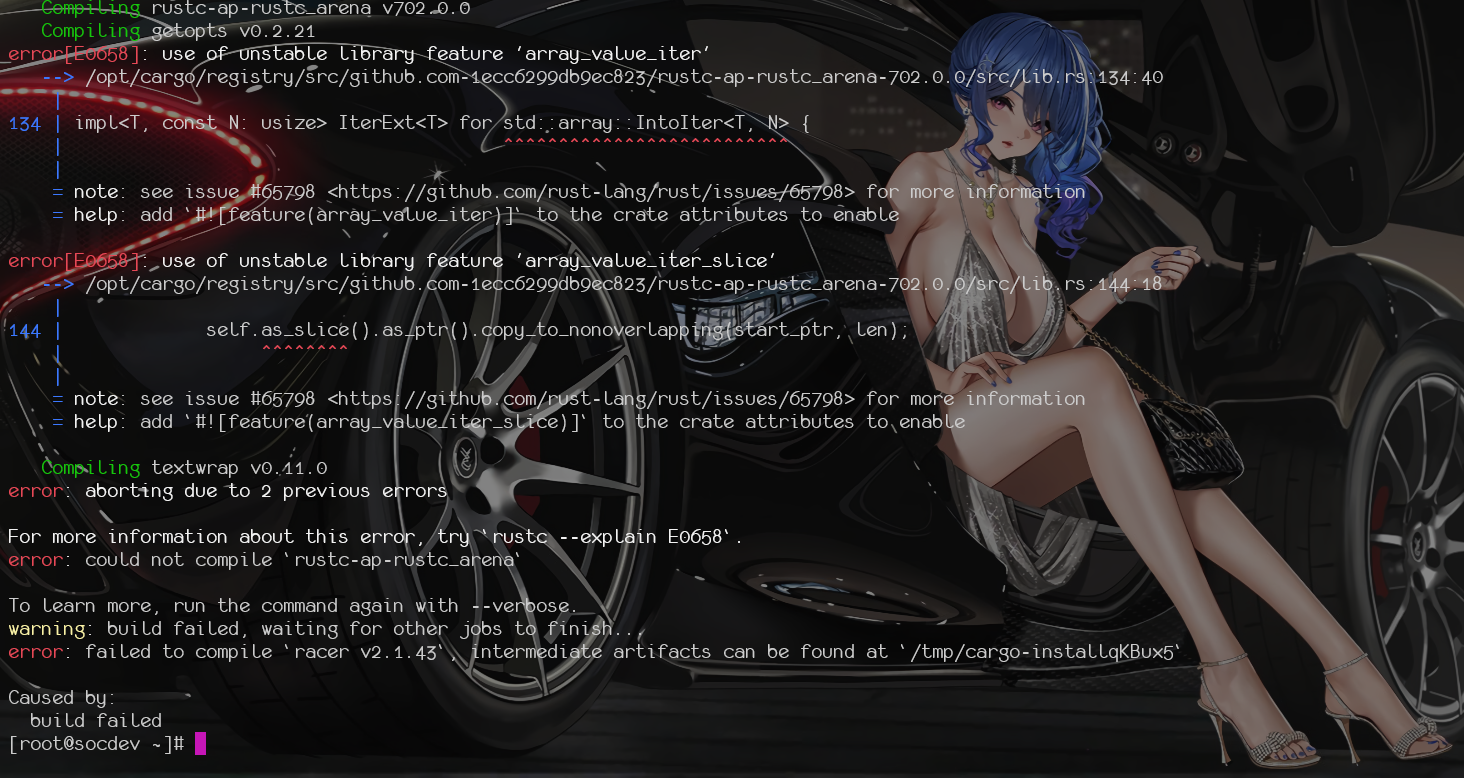
\includegraphics[width=\linewidth]{rust_feature_error.png}
  \caption{缺少特性支持编译失败}
  \label{fig:rust_feature_error}
\end{figure}
遇到这种错误,则需要直接修改对应的类库的源代码。以上述错误为例,编译的help表示
\mintinline[breaklines=true,breakanywhere,breaksymbolleft=,breakanywheresymbolpre=,]{bash}{add `#![feature(array_value_iter_slice)]` to the crate attributes to enable},
则我们应当在对应的crate的lib.rs的头部当中,添加内容如下:
\begin{figure}[H]
  \centering
  
\includegraphics[width=\linewidth]{rust_feature_add.png}
  \caption{增加特性支持}
  \label{fig:rust_feature_add}
\end{figure}
